\documentclass[UTF8,10pt,a4paper]{ctexart}

\usepackage[top=1in, bottom=1in, left=1in, right=1in]{geometry}
\usepackage{indentfirst}
\usepackage{setspace}
\usepackage{color}

%font
\usepackage{fontspec,xltxtra,xunicode}
\setromanfont{STZhongsong}

%section
\ctexset{section/format=\Large\bfseries}


%table
\usepackage{threeparttable} %表格注释
\usepackage{diagbox} % 单元格斜线
\usepackage{multicol}
\usepackage{multirow}
\usepackage{booktabs} %toprule...
\usepackage{arydshln} %虚线
\usepackage{dashrule} %虚线

%list


%figs
\usepackage{graphicx}
\usepackage{subfigure}
\usepackage{float}
\graphicspath{{./figs/}{./}{./figs2/}}

%logo
\usepackage{fancyhdr}
\pagestyle{fancy}
\lhead{\includegraphics[scale=0.1]{BGIlogo.png}}  %在此处插入logo.pdf图片

%附录&副标题
\usepackage[titletoc]{appendix}
\usepackage{titling}
\newcommand{\subtitle}[1]{%
  \posttitle{%
    \par\end{center}
    \begin{center}\small#1\end{center}
    \vskip0.5em}%
}

%超链接
%\usepackage[hyperfootnotes=true]{hyperref}
\usepackage[colorlinks,
            linkcolor=red,
            anchorcolor=blue,
            citecolor=green,
            urlcolor=blue]{hyperref}

%原文照列
\usepackage{verbatim}
\usepackage{clrscode}
\usepackage{listings} %插入代码

\lstset{numbers=left, %设置行号位置
        backgroundcolor=\color[RGB]{245,245,244},
        basicstyle=\footnotesize,
        showstringspaces=false,
        numberstyle=\tiny, %设置行号大小
        keywordstyle=\color{blue}, %设置关键字颜色
        commentstyle=\color[cmyk]{1,0,1,0}, %设置注释颜色
        frame=single, %设置边框格式
   %     escapeinside=``, %逃逸字符(1左面的键),用于显示中文
       basicstyle=\scriptsize\ttfamily,
        breaklines, %自动折行
        extendedchars=false, %解决代码跨页时,章节标题,页眉等汉字不显示的问题
        xleftmargin=2em,xrightmargin=2em, aboveskip=1em, %设置边距
        tabsize=4, %设置tab空格数
        showspaces=false, %不显示空格
        %belowcaptionskip=1\baselineskip,
        stringstyle=\color{orange}
        }

\title{NGS分析流程性能及准确度评估{\small (v0.3)}}
\subtitle{Edited from 《edico性能及准确度评估{\small (v0.2)}》}
\author{\href{http://bigdata.genomics.cn/}{大数据计算组} \and
\href{mailto:huangzhibo@genomics.cn}{马强华}}
\date{\today}

%\author{\textcolor{blue}{huangzhibo@genomics.cn}

\begin{document}
\maketitle
\vspace{3em}
%\tableofcontents
\setcounter{tocdepth}{2}
\tableofcontents\thispagestyle{empty}
\newpage
\setlength{\parskip}{1ex plus 0.5ex minus 0.2ex}


%\setcounter{subsection}{0}

\section{目的}
对比评估NGS分析流程的性能及其变异检测精度(snp \& indel突变类型)。

\section{说明}

\subsection{数据}
\begin{enumerate}
%\item XtenHiseq NA12878 \\
%	数据信息
\item Zebra500 NA12878 38X
{\footnotesize
\begin{itemize}
\item /hwfssz1/BIGDATA\_COMPUTING/data/NA12878/Zebra500\_NA12878\_WGS/NA12878\_read\_1.fq.gz
\item /hwfssz1/BIGDATA\_COMPUTING/data/NA12878/Zebra500\_NA12878\_WGS/NA12878\_read\_2.fq.gz
\end{itemize}
}
\end{enumerate}

\subsection{reference版本}
hg19

\subsection{分析流程及所用计算资源}
\begin{enumerate}

\item GATK3
	\begin{itemize}
	\item 说明 : 即GATK Best Practices(GATK3.7)
	\item 计算节点:cngb-hadoop-a16-4(10.53.20.164)\\
	 CPU: Intel(R) Xeon(R) CPU E5-2650 v4 @ 2.20GHz, CPU核数 : 12,  逻辑CPU: 48\\
	 内存: 256G
	\end{itemize}
\item GATK3\_2 
	\begin{itemize}
	\item 说明:使用biobambam2 bamsormadup作为排序去重工具,其他步骤同GATK Best Practices
	\item 计算节点:cngb-compute-e03-9 (10.53.0.39)\\
	 CPU: Intel(R) Xeon(R) CPU E7-4830 v4 @ 2.00GHz, CPU核数 : 14,  逻辑CPU: 112\\
	 内存: 512G
	\end{itemize}
\item GATK4
	\begin{itemize}
	\item 说明 : beta版本
	 \item 计算节点:同GATK3
	\end{itemize}
\item GaeaHC : Gaea + hadoop streaming GATK HC
	\begin{itemize}
	\item 计算节点: 10.53.20.[12-32]共20个计算节点\\
	 CPU: Intel(R) Xeon(R) CPU E5-2650 v4 @ 2.20GHz, CPU核数 : 12,  逻辑CPU: 48\\
	 内存: 256G
	\end{itemize}
\item edico
      \begin{itemize}
      \item 计算节点:cngb-edico-a23-1 (10.53.4.148)\\
         CPU: Intel(R) Xeon(R) CPU E5-2690 v4 @ 2.60GHz, CPU核数 : 14,  逻辑CPU: 56\\
	 内存: 256G
	\end{itemize}
\item Sentieon
\begin{itemize}
\item 计算节点: 同GATK3
\end{itemize}
\begin{description}
\item[注1:]  各流程所使用变异检测算法均为 HaplotyperCaller,均不对vcf结果做额外处理(矫正过滤等)。
\item[注2:]  存储均使用:华为os9000 (/hwfssz1/BIGDATA\_COMPUTING)
\end{description}
\end{enumerate}

\section{性能评估}
\subsection{各流程耗时}
\begin{table}[htp]
\newcommand{\tabincell}[2]{\begin{tabular}{@{}#1@{}}#2\end{tabular}}
{\small
\caption{各流程耗时}
\begin{center}
\begin{threeparttable}
\begin{tabular}{p{2cm}|p{2cm}|p{2cm}|p{2cm}|p{2cm}|p{2cm}|p{2cm}}
\hline
\diagbox[width=7.5em]{步骤}{流程} & GATK4 &  GATK3\tnote{1} & GATK3\_2\tnote{2}& GaeaHC\tnote{3} & Sentieon & edico \\
\hline
比对 & 04:01:02 & 04:01:02 & 04:41:10 & 00:19:49 & 04:08:36 & -\\
排序和去重 & 14:16:59 & 14:16:59 & 0 & 00:06:10&  00:30:11 & -\\
重比对  & 0 & 0 & 0 & 0 & 00:21:15 & -\\
质量值矫正 & 05:57:02 & 02:38:17 & 02:41:46 &  00:12:56 &  01:51:44 & - \\
PrintRead & 05:52:13  & 15:26:21 & 26:20:33 & 0 & 0 & -\\
变异检测 & 08:27:55 & 14:59:22 & 08:41:08 & 00:26:00 & 00:41:33 & -\\
总计 & 38:59:33 &  41:22:02 & 42:24:37 & 01:05:00 & 07:33:19 & 00:36:00\\
\hline
\end{tabular}

      \begin{tablenotes}
        \footnotesize
        \item[1] {\kaishu GATK3的BaseRecalibrator处理的数据来源于GATK4的MarkDuplicates处理后得到的bam文件数据}
        \item[2] {\kaishu 该流程过滤耗时包含在比对步骤中}
        \item[3] {\kaishu 不包含解压步骤}
      \end{tablenotes}
\end{threeparttable}
\end{center}
}
\end{table}

%\begin{table}[htp]
%\newcommand{\tabincell}[2]{\begin{tabular}{@{}#1@{}}#2\end{tabular}}
%{\small
%\caption{Sentieon各流程总耗时}
%\begin{center}
%\begin{tabular}{p{5cm}|p{5cm}}
%\hline
%流程 & 小时:分钟:秒 \\
%\hline
%BWA &  \\
%Metrics & 00:08:40 \\
%Dedup & 00:21:31 \\
%Indel re-aligner & 00:21:15 \\
%BSQR & 01:51:44 \\
%Variant & 00:41:33 \\
%总计 & 07:33:19 \\
%\hline
%\end{tabular}
%\end{center}
%\label{default}
%}
%\end{table}

\section{变异检测精度评估}
\subsection{精度评估软件及指标说明}
\begin{enumerate}
\item 评估软件
\begin{itemize}
\item RTG vcfeval
\end{itemize}
\item \href{https://note.youdao.com/share/?token=170F71A3F2494D089B29E2AD944A6ECA&gid=12269890}{评估指标说明}
\begin{itemize}
\item 真阳性位点(True positives)  :  在标准集中存在,test.vcf中也存在的变异数。 
\item 假阴性位点(False negatives):  在标准集中存在,test.vcf中不存在的变异数。
\item 假阳性位点(False positives) :  在标准集中不存在, test.cf中存在的变异数。
%\end{itemize}
%\item 计算公式
%\begin{itemize}
\item Precision (PPV) 		: (true positives) / (true positives + false positives) 
\item Recall (sensitivity)		: (true positives) / (true positives + false negatives) 
\item F-measure			: 2 * precision * recall / (precision + recall)
\end{itemize}
\end{enumerate}
根据F-measure(Precision和Recall的调和平均数)的值来判断结果优劣,值越高越好。\\
Threshold是变异的QUAL值,作为结果最优情况下的过滤阈值。

\subsection{snp评估}
\subsubsection{评估指标数值}
\begin{table}[htp]
\newcommand{\tabincell}[2]{\begin{tabular}{@{}#1@{}}#2\end{tabular}}
{\small
\caption{各流程评估指标}
\begin{center}
\begin{threeparttable}
\begin{tabular}{p{1.5cm}|p{1.5cm}|p{1.5cm}|p{1.5cm}|p{1.5cm}|p{1.5cm}|p{1.5cm}|p{1.7cm}}
\hline
\diagbox[width=6em]{流程}{评估指标} & Threshold\tnote{1} & True-pos & False-pos & False-neg & Precision & Sensitivity & F-measure\\
\hline
GATK3 & 47.280 & 3176500 & 19675 & 16449 & 0.9938 & 0.9948  & 0.9943\\
GATK3\_2 & 47.280 & 3176487 & 19672 & 16462 & 0.9938 & 0.9948 & 0.9943 \\
GATK4 & 49.790 & 3176298 & 19676 & 16651 & 0.9938 & 0.9948  & 0.9943\\
GaeaHC & 50.740 & 3176310 & 19902 & 16639 & 0.9938 & 0.9948 & 0.9943 \\
edico & 37.860 & 3176461 & 19765 & 16488 & 0.9938 & 0.9948 & 0.9943 \\
Sentieon & 50.740 & 3176222 & 19434 & 16727 & 0.9939 & 0.9948  & 0.9943\\
\hline
\end{tabular}
\begin{tablenotes}
\item[1] {\kaishu 根据QUAL阈值,取F-measure最大时的值}
\end{tablenotes}
\end{threeparttable}
\end{center}
}
\end{table}

\subsubsection{snp精度ROC曲线图}
\begin{figure}[htb]
\begin{center}
\begin{threeparttable}
\label{snp}
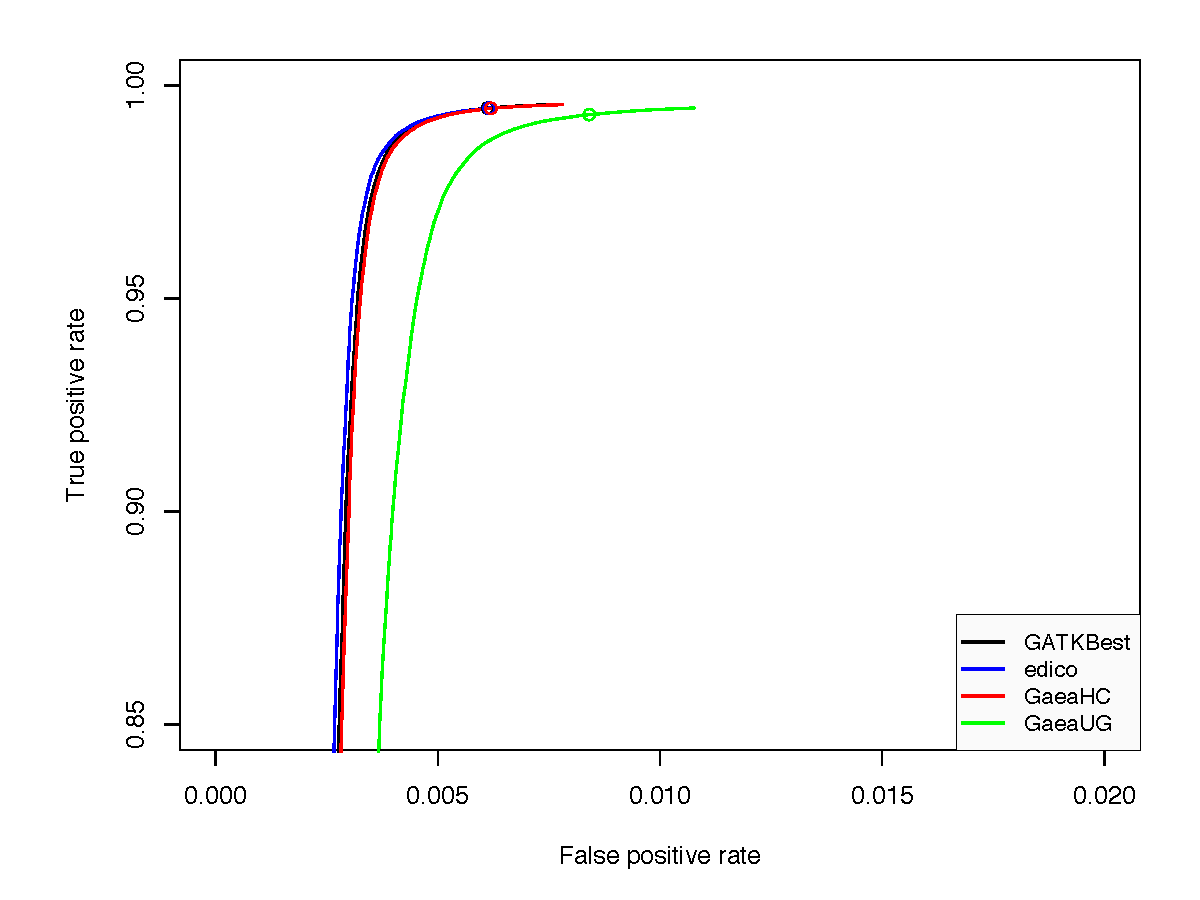
\includegraphics[width=15cm]{snp.pdf}
\caption{ROC曲线图}
\begin{tablenotes}
\item[1] {\kaishu 该ROC曲线根据QUAL值绘制}
\item[2] {\kaishu 曲线上圆圈位置为F-measure最大时的QUAL值}
\end{tablenotes}
\end{threeparttable}
\end{center}
\end{figure}
%{\color{cyan}{\small \kaishu{Gaea + GATK HC:}}}
\subsubsection{snp评估结论}
	各流程在snp上的结果F-measure均相同,其精度没有明显差异。

\subsection{indel评估}
\subsubsection{评估指标数值}
\begin{table}[htp]
\newcommand{\tabincell}[2]{\begin{tabular}{@{}#1@{}}#2\end{tabular}}
{\small
\caption{各流程评估指标}
\begin{center}
\begin{threeparttable}
\begin{tabular}{p{1.5cm}|p{1.5cm}|p{1.5cm}|p{1.5cm}|p{1.5cm}|p{1.5cm}|p{1.5cm}|p{1.7cm}}
\hline
\diagbox[width=6em]{流程}{评估指标} & Threshold\tnote{1} & True-pos & False-pos & False-neg & Precision & Sensitivity & F-measure\\
\hline
GATKBest & 59.770 & 356685 & 14100 & 12794 & 0.9620 & 0.9654 & 0.9637 \\
edico & 73.200 & 355273 & 14789 & 14206 & 0.9600 & 0.9616 & 0.9608 \\
GaeaHC & 73.730 & 356105 & 14437 & 13374 & 0.9610 & 0.9638 & 0.9624 \\
GATK3 & 59.770 & 356685 & 14103 & 12794 & 0.9620 & 0.9654  & 0.9637\\
GATK4 & 73.730 & 356042 & 14345 & 13437 & 0.9613 & 0.9636  & 0.9624\\
Sentieon &  59.770 & 355874 & 14674 & 13605 & 0.9604 & 0.9632  & 0.9618\\
\hline
\end{tabular}
\begin{tablenotes}
\item[1] {\kaishu 根据QUAL阈值,取F-measure最大时的值}
\end{tablenotes}
\end{threeparttable}
\end{center}
}
\end{table}

\subsubsection{indel精度ROC曲线图}
\begin{figure}[htb]
\begin{center}
\begin{threeparttable}
\label{indel}
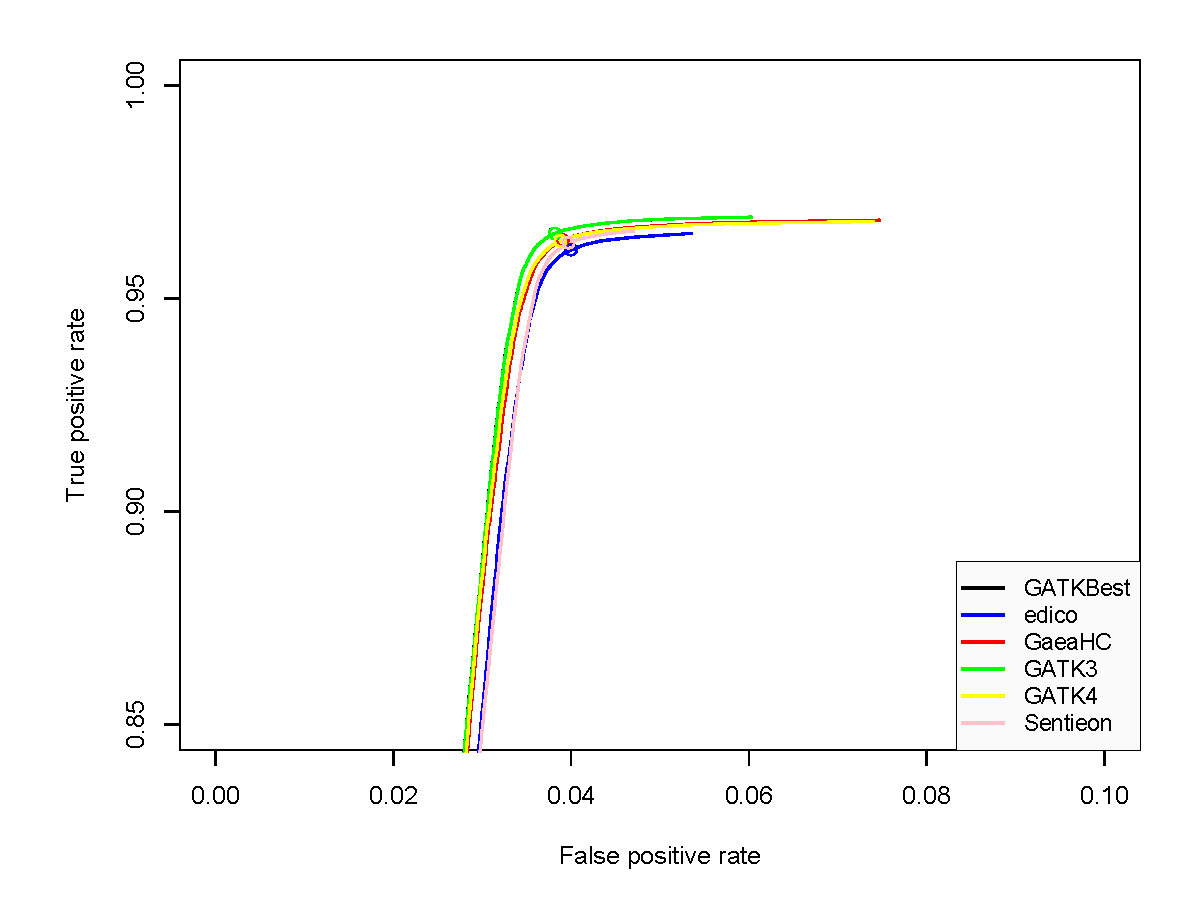
\includegraphics[width=15cm]{indel.pdf}
\caption{ROC曲线图}
\begin{tablenotes}
\item[1] {\kaishu 该ROC曲线根据QUAL值绘制}
\item[2] {\kaishu 曲线上圆圈位置为F-measure最大时的QUAL值}
\end{tablenotes}
\end{threeparttable}
\end{center}
\end{figure}
\subsubsection{indel评估结论}
	GATK3流程在indel检测上结果最优,edico最差。

%\subsection{cnv评估}
%暂缺

\section{总结}
edico性能最好,用时只有36分钟。各流程在snp的检测上差异很微小,从indel结果看GATK3流程精度最优,edico最差。总体看,结果相差并不很大,在可接受范围内。

\end{document}
